\documentclass[border=3pt]{standalone}
% Preâmbulo compartilhado pelos diagramas TikZ da aula 13 (SLAM com EKF)
\usepackage[T1]{fontenc}
\usepackage[utf8]{inputenc}
\usepackage{lmodern}
\usepackage{amsmath}
\usepackage{xcolor}
\usepackage{tikz}
\usetikzlibrary{arrows.meta,angles,quotes,decorations.pathmorphing,decorations.pathreplacing,calc,
                positioning,shapes.geometric,shapes.misc,backgrounds,fit,
                math}

% Paleta (mesma dos SVGs originais)
\definecolor{dblue}{HTML}{2A5B8C}
\definecolor{dorange}{HTML}{B3541E}
\definecolor{dgreen}{HTML}{4A7C59}
\definecolor{dred}{HTML}{9C4B4B}
\definecolor{dcream}{HTML}{F4F1EA}
\definecolor{dshade}{HTML}{DDD7C9}

% Função gaussiana (não normalizada por padrão de escala visual)
\pgfmathdeclarefunction{gauss}{3}{%
  \pgfmathparse{1/(#3*sqrt(2*pi))*exp(-((#1-#2)^2)/(2*#3^2))}%
}

% Estilos comuns (prefixo d... para não colidir com chaves internas do pgf)
\tikzset{
  >={Stealth[length=2mm]},
  dguide/.style={gray!55, dashed, line width=0.4pt},
  daxis/.style={gray!60, line width=0.7pt, ->},
  dbody/.style={fill=black!3, draw=black!80, line width=1pt},
  dacc/.style={draw=dblue, line width=1pt},
  dlbl/.style={black!55, font=\small},
  dsub/.style={black!45, font=\footnotesize},
  dstate/.style={circle, draw=black!80, fill=dcream, line width=1pt,
                 minimum size=17mm, font=\large, inner sep=1pt},
  dobs/.style={circle, draw=black!80, fill=dshade, line width=1pt,
               minimum size=14mm, font=\large, inner sep=1pt},
  dbox/.style={rounded corners=2pt, draw=black!80, fill=dcream, line width=1pt,
               align=center, inner sep=6pt},
  dop/.style={circle, draw=black!80, fill=white, line width=1pt,
              minimum size=6mm, inner sep=0pt, font=\small},
  dtrans/.style={->, dblue, line width=1pt},
  dmeas/.style={->, dorange, line width=1pt},
  dcurve/.style={line width=1pt, dblue},
  dcurveb/.style={line width=1.4pt, dorange},
}

\begin{document}
\hyphenpenalty=10000 \exhyphenpenalty=10000 \tolerance=9999 \emergencystretch=3em
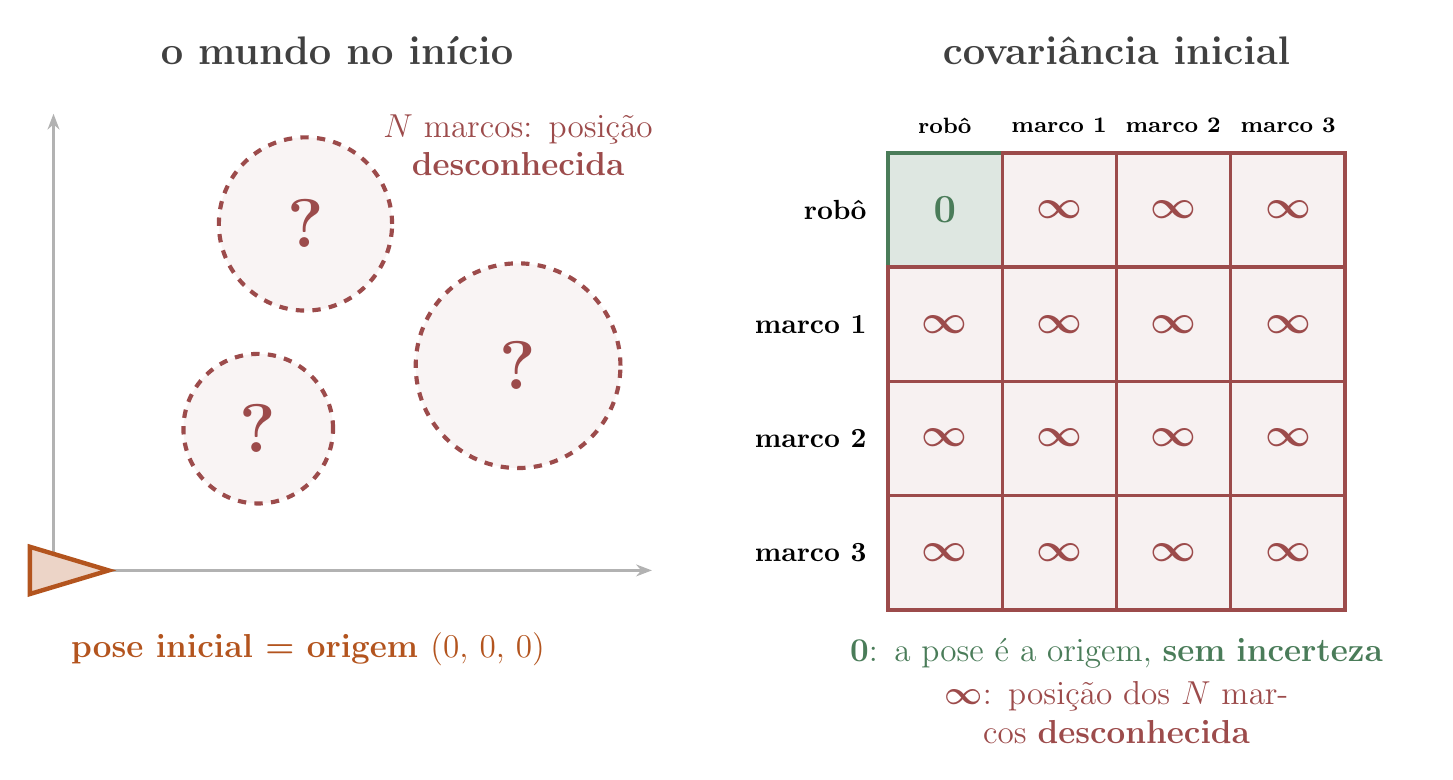
\begin{tikzpicture}[x=1cm,y=1cm]
\node[font=\Large\bfseries, black!75] at (4.6,8.6) {o mundo no início};
\draw[daxis, line width=1.2pt] (1.0,2.0) -- (8.6,2.0); \draw[daxis, line width=1.2pt] (1.0,2.0) -- (1.0,7.8);
\draw[dorange, fill=dorange!25, line width=1.6pt] (0.7,1.7) -- (1.7,2.0) -- (0.7,2.3) -- cycle;
\node[font=\large\bfseries, dorange, anchor=west] at (1.1,1.0) {pose inicial = origem $(0,\,0,\,0)$};
\draw[dred, dashed, fill=dred!6, line width=1.5pt] (4.2,6.4) circle (1.1);
\node[font=\Huge\bfseries, dred] at (4.2,6.4) {?};
\draw[dred, dashed, fill=dred!6, line width=1.5pt] (6.9,4.6) circle (1.3);
\node[font=\Huge\bfseries, dred] at (6.9,4.6) {?};
\draw[dred, dashed, fill=dred!6, line width=1.5pt] (3.6,3.8) circle (0.95);
\node[font=\Huge\bfseries, dred] at (3.6,3.8) {?};
\node[font=\large, dred, text width=4.2cm, align=center] at (6.9,7.4) {$N$ marcos: posição \textbf{desconhecida}};
\node[font=\Large\bfseries, black!75] at (14.5,8.6) {covariância inicial};
\node[font=\normalsize\bfseries, anchor=east] at (11.45,6.58) {robô};
\node[font=\footnotesize\bfseries] at (12.32,7.65) {robô};
\draw[dgreen, fill=dgreen!18, line width=1.3pt] (11.6,7.3) rectangle (13.05,5.85);
\node[font=\Large, text=dgreen] at (12.32,6.58) {\textbf{0}};
\draw[dred, fill=dred!8, line width=1.3pt] (13.05,7.3) rectangle (14.5,5.85);
\node[font=\Large, text=dred] at (13.77,6.58) {$\boldsymbol{\infty}$};
\draw[dred, fill=dred!8, line width=1.3pt] (14.5,7.3) rectangle (15.95,5.85);
\node[font=\Large, text=dred] at (15.22,6.58) {$\boldsymbol{\infty}$};
\draw[dred, fill=dred!8, line width=1.3pt] (15.95,7.3) rectangle (17.4,5.85);
\node[font=\Large, text=dred] at (16.68,6.58) {$\boldsymbol{\infty}$};
\node[font=\normalsize\bfseries, anchor=east] at (11.45,5.12) {marco 1};
\node[font=\footnotesize\bfseries] at (13.77,7.65) {marco 1};
\draw[dred, fill=dred!8, line width=1.3pt] (11.6,5.85) rectangle (13.05,4.4);
\node[font=\Large, text=dred] at (12.32,5.12) {$\boldsymbol{\infty}$};
\draw[dred, fill=dred!8, line width=1.3pt] (13.05,5.85) rectangle (14.5,4.4);
\node[font=\Large, text=dred] at (13.77,5.12) {$\boldsymbol{\infty}$};
\draw[dred, fill=dred!8, line width=1.3pt] (14.5,5.85) rectangle (15.95,4.4);
\node[font=\Large, text=dred] at (15.22,5.12) {$\boldsymbol{\infty}$};
\draw[dred, fill=dred!8, line width=1.3pt] (15.95,5.85) rectangle (17.4,4.4);
\node[font=\Large, text=dred] at (16.68,5.12) {$\boldsymbol{\infty}$};
\node[font=\normalsize\bfseries, anchor=east] at (11.45,3.68) {marco 2};
\node[font=\footnotesize\bfseries] at (15.22,7.65) {marco 2};
\draw[dred, fill=dred!8, line width=1.3pt] (11.6,4.4) rectangle (13.05,2.95);
\node[font=\Large, text=dred] at (12.32,3.68) {$\boldsymbol{\infty}$};
\draw[dred, fill=dred!8, line width=1.3pt] (13.05,4.4) rectangle (14.5,2.95);
\node[font=\Large, text=dred] at (13.77,3.68) {$\boldsymbol{\infty}$};
\draw[dred, fill=dred!8, line width=1.3pt] (14.5,4.4) rectangle (15.95,2.95);
\node[font=\Large, text=dred] at (15.22,3.68) {$\boldsymbol{\infty}$};
\draw[dred, fill=dred!8, line width=1.3pt] (15.95,4.4) rectangle (17.4,2.95);
\node[font=\Large, text=dred] at (16.68,3.68) {$\boldsymbol{\infty}$};
\node[font=\normalsize\bfseries, anchor=east] at (11.45,2.23) {marco 3};
\node[font=\footnotesize\bfseries] at (16.68,7.65) {marco 3};
\draw[dred, fill=dred!8, line width=1.3pt] (11.6,2.95) rectangle (13.05,1.5);
\node[font=\Large, text=dred] at (12.32,2.23) {$\boldsymbol{\infty}$};
\draw[dred, fill=dred!8, line width=1.3pt] (13.05,2.95) rectangle (14.5,1.5);
\node[font=\Large, text=dred] at (13.77,2.23) {$\boldsymbol{\infty}$};
\draw[dred, fill=dred!8, line width=1.3pt] (14.5,2.95) rectangle (15.95,1.5);
\node[font=\Large, text=dred] at (15.22,2.23) {$\boldsymbol{\infty}$};
\draw[dred, fill=dred!8, line width=1.3pt] (15.95,2.95) rectangle (17.4,1.5);
\node[font=\Large, text=dred] at (16.68,2.23) {$\boldsymbol{\infty}$};
\node[font=\large, dgreen, text width=7.6cm, align=center] at (14.5,0.95) {\textbf{0}: a pose é a origem, \textbf{sem incerteza}};
\node[font=\large, dred, text width=7.6cm, align=center] at (14.5,0.2) {$\boldsymbol{\infty}$: posição dos $N$ marcos \textbf{desconhecida}};
\end{tikzpicture}
\end{document}
